% Copyright 2022 by Marek Rychly <rychly@fit.vut.cz>.
%
\documentclass[10pt,xcolor=pdflatex,dvipsnames,table,oneside]{book}
% babel and encoding
\usepackage[czech]{babel}
\usepackage[T1]{fontenc}
\usepackage[utf8]{inputenc}
\usepackage{lmodern}

\usepackage{csquotes}% correct/formal language-specific quotations
\usepackage{microtype}% character protrusion, font expansion, adjustment of interword spacing, additional kerning, tracking, etc.
\usepackage{hyperref}% hyper-refs in PDF
\usepackage{graphicx}

\author{
    František Koleček, \href{mailto:xkolec08@stud.fit.vut.cz}{xkolec08@stud.fit.vut.cz} \\
    Tomáš Moravčík, \href{mailto:xmorav41@stud.fit.vut.cz}{xmorav41@stud.fit.vut.cz} \\
    David Sladký, \href{mailto:xsladk07@stud.fit.vut.cz}{xsladk07@stud.fit.vut.cz}
    }
\title{Příprava dat a jejich popisná charakteristika}
\date{zima 2022}

\begin{document}

\pagenumbering{roman}

\hypersetup{pageanchor=false}% disable hyperref anchor to title page as maketitle enforce pagenumbering to arabic which colides the titlepage with the first arabic page below
\maketitle
\hypersetup{pageanchor=true}

\tableofcontents

\newpage% force page-break to start the page numbering on a new page
\pagenumbering{arabic}

% DOKUMENTACE K PRVNI CASTI DRUHEHO PROJEKTU
\chapter{Explorativní analýza}

\section{Zadání}

\verb|penguins_size.csv| je datová sada obsahující údaje o populaci tučnáků na ostrovech u pobřeží Antarktidy. Cílem
této části je provést explorativní analýzu, neboli prozkoumaní atributů datové sady a jejich rozložení, odhalit odlehlé a chybějící
hodnoty a provést korelační analýzu.

\section{Nástroje}
Pro prozkoumání datové sady byl zvolen programovací jazyk Python. Konrétně byly využity knihovny pandas, matplotlib a seaborn.
Tyhle knihovny je možné doinstalovat příkazem \verb|pip install pandas matplotlib seaborn|. Script provádějící explorativní
analýzu je uloženv souboru \verb|src/exploration.py|, který na svém vyžaduje jeden parametr a to cestu k datasetu. Tento
skript vydává textový výstup, tak i řadu grafů. \

Příklad spuštění: \

\verb|python3 ./src/exploration.py ./dataset/penguins_size.csv|\

Nebo pomocí Makefile: \

\verb|make exp|\

\section{Prozkoumání atributů datové sady}

\subsubsection{Základní popis kategorických atributů.}
\vspace{1em}
\begin{tabular}{|l|l|l|l|}
    \hline
    & Druh & Ostrov & Pohlaví \\
    \hline
    \hline
    Počet & 344 & 344 & 334 \\
    \hline
    Unikátních & 3 & 3 & 3 \\
    \hline
    Nejčastější & Adelie & Biscoe & MALE \\
    \hline
    Frekvence & 152 & 168 & 168 \\
    \hline
\end{tabular}

\subsubsection{Počet jedinců jednotlivých druhů.}
\vspace{1em}
\begin{tabular}{|l|l|l|}
    \hline
    Jméno & Počet & Zastoupení \\
    \hline
    \hline
    Adelie & 152 & 44.2\% \\
    \hline
    Gentoo & 124 & 36.0\% \\
    \hline
    Chinstrap & 68 & 19.8\% \\
    \hline
\end{tabular}

\subsubsection{Počet tučňáků na jednotlivých ostrovech}
\vspace{1em}
\begin{tabular}{|l|l|l|}
    \hline
    Jméno & Počet & Zastoupení \\
    \hline
    \hline
    Biscoe    & 168 & 48.8\% \\
    \hline
    Dream     & 124 & 36.0\% \\
    \hline
    Torgersen & 52 & 15.1\% \\
    \hline
\end{tabular}

\subsubsection{Rozložení pohlaví tůčňáků}
\vspace{1em}
\begin{tabular}{|l|l|l|}
    \hline
    Pohlaví & Počet & Zastoupení \\
    \hline
    \hline
    MALE    & 168 & 50.3\% \\
    \hline
    FEMALE     & 165 & 49.4\% \\
    \hline
    . & 1 & 0.3\% \\
    \hline
\end{tabular}

\subsubsection{Vlastnosti číselných atributů}
\vspace{1em}
\begin{tabular}{|l|l|l|l|l|}
    \hline
    & culmen length mm & culmen depth mm & flipper length mm & body mass g \\
    \hline
    \hline
    count  & 342.00 & 342.00 & 342.00 &  342.00 \\
    \hline
    mean   &  43.92 &  17.15 & 200.91 & 4201.75 \\
    \hline
    std    &   5.45 &   1.97 &  14.06 &  801.95 \\
    \hline
    min    &  32.10 &  13.10 & 172.00 & 2700.00 \\
    \hline
    25\%   &  39.22 &  15.60 & 190.00 & 3550.00 \\
    \hline
    50\%   &  44.45 &  17.30 & 197.00 & 4050.00 \\
    \hline
    75\%   &  48.50 &  18.70 & 213.00 & 4750.00 \\
    \hline
    max    &  59.60 &  21.50 & 231.00 & 6300.00 \\
    \hline
\end{tabular}

\section{Rozložení atributů}

\subsubsection{Zastoupení jednotlivých druhů na ostrovech}
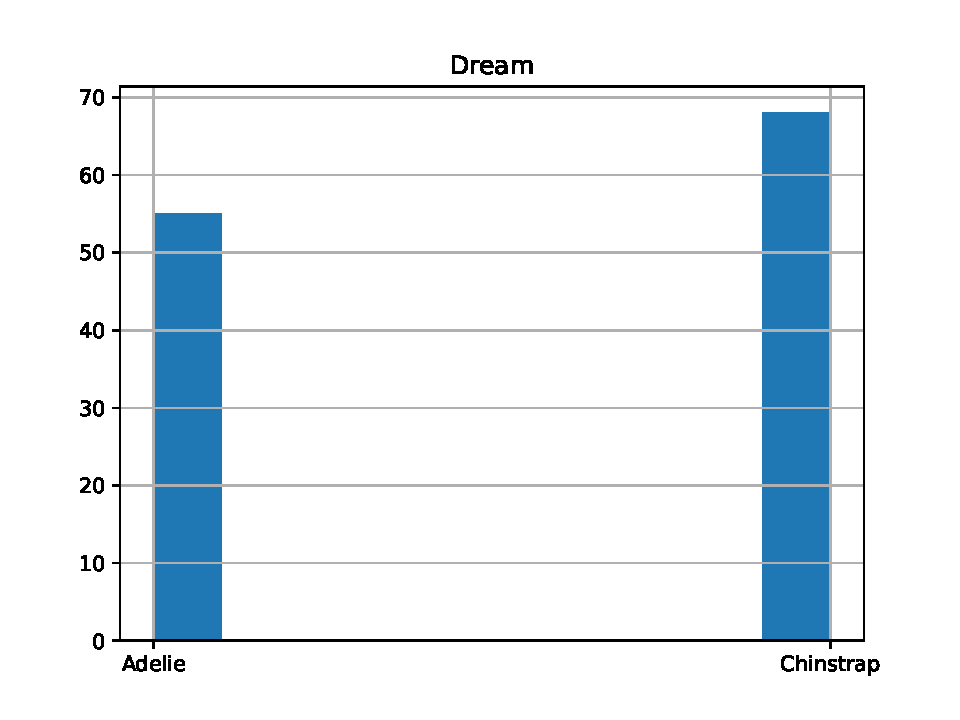
\includegraphics[width=0.5\textwidth, angle = 0]{img/dream-species.pdf}
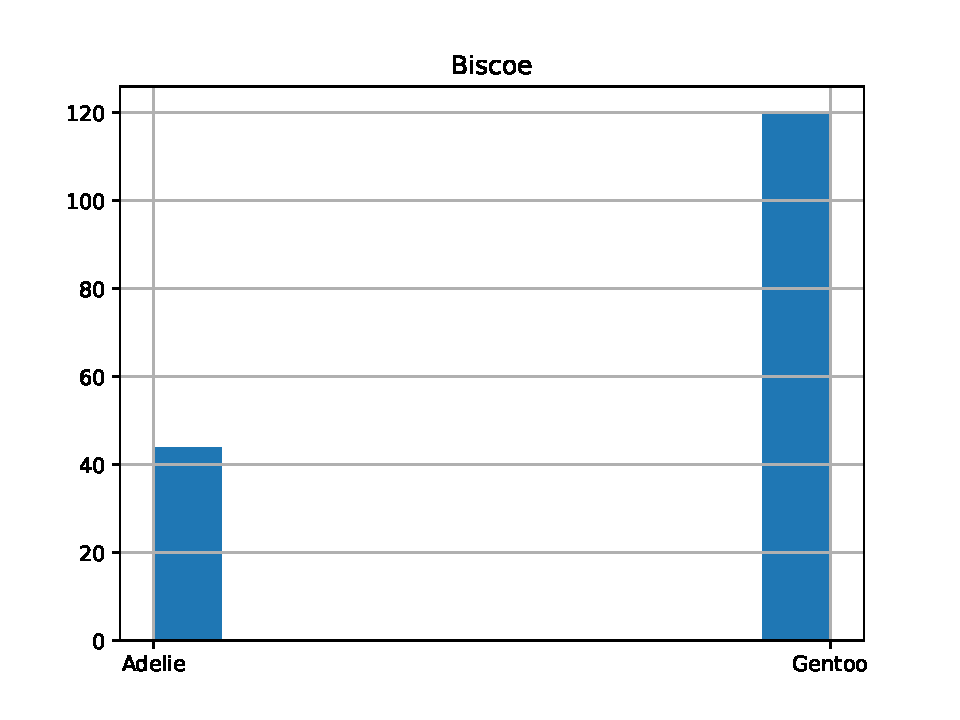
\includegraphics[width=0.5\textwidth, angle = 0]{img/biscoe-species.pdf}
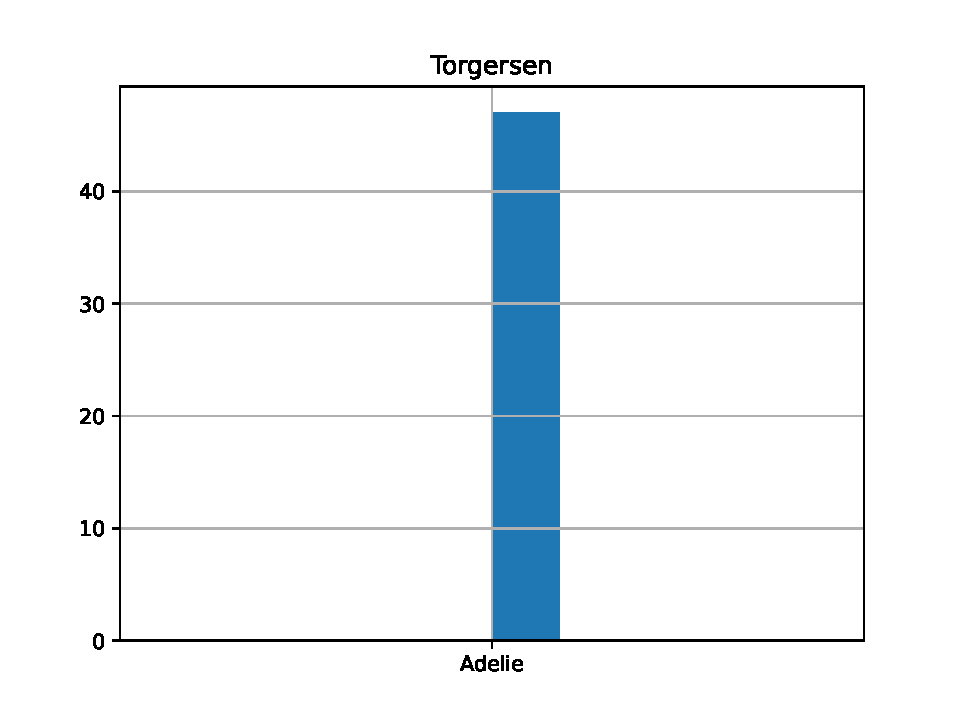
\includegraphics[width=0.5\textwidth, angle = 0]{img/torgersen-species.pdf}


\subsubsection{Rozložení numerických atributů v závisloti na pohlaví a druhu}
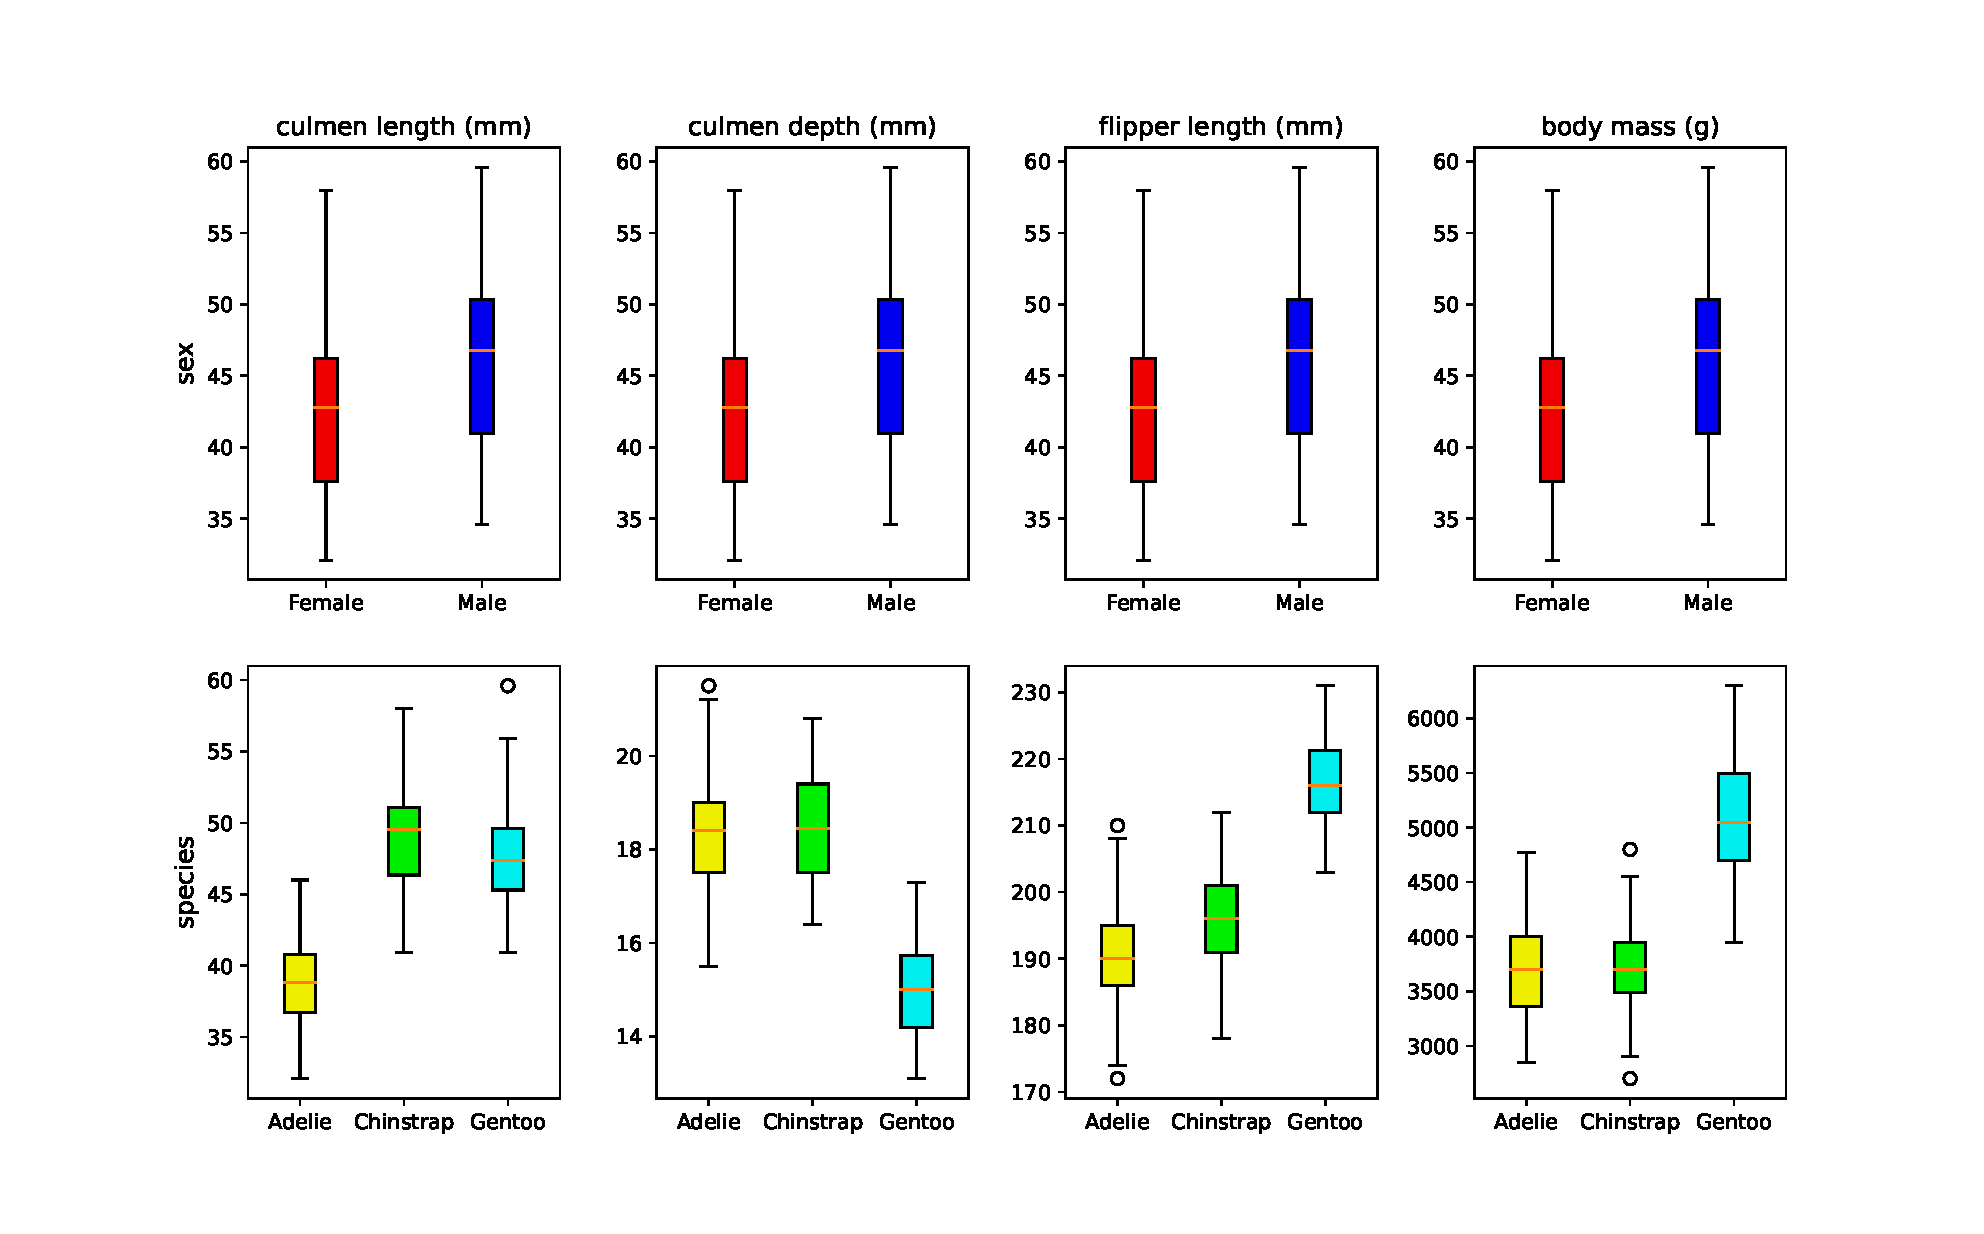
\includegraphics[width=1.0\textwidth, angle = 0]{img/box.pdf}

\subsubsection{Podrobnější rozložení numerických atributů v závisloti na pohlaví - Female}
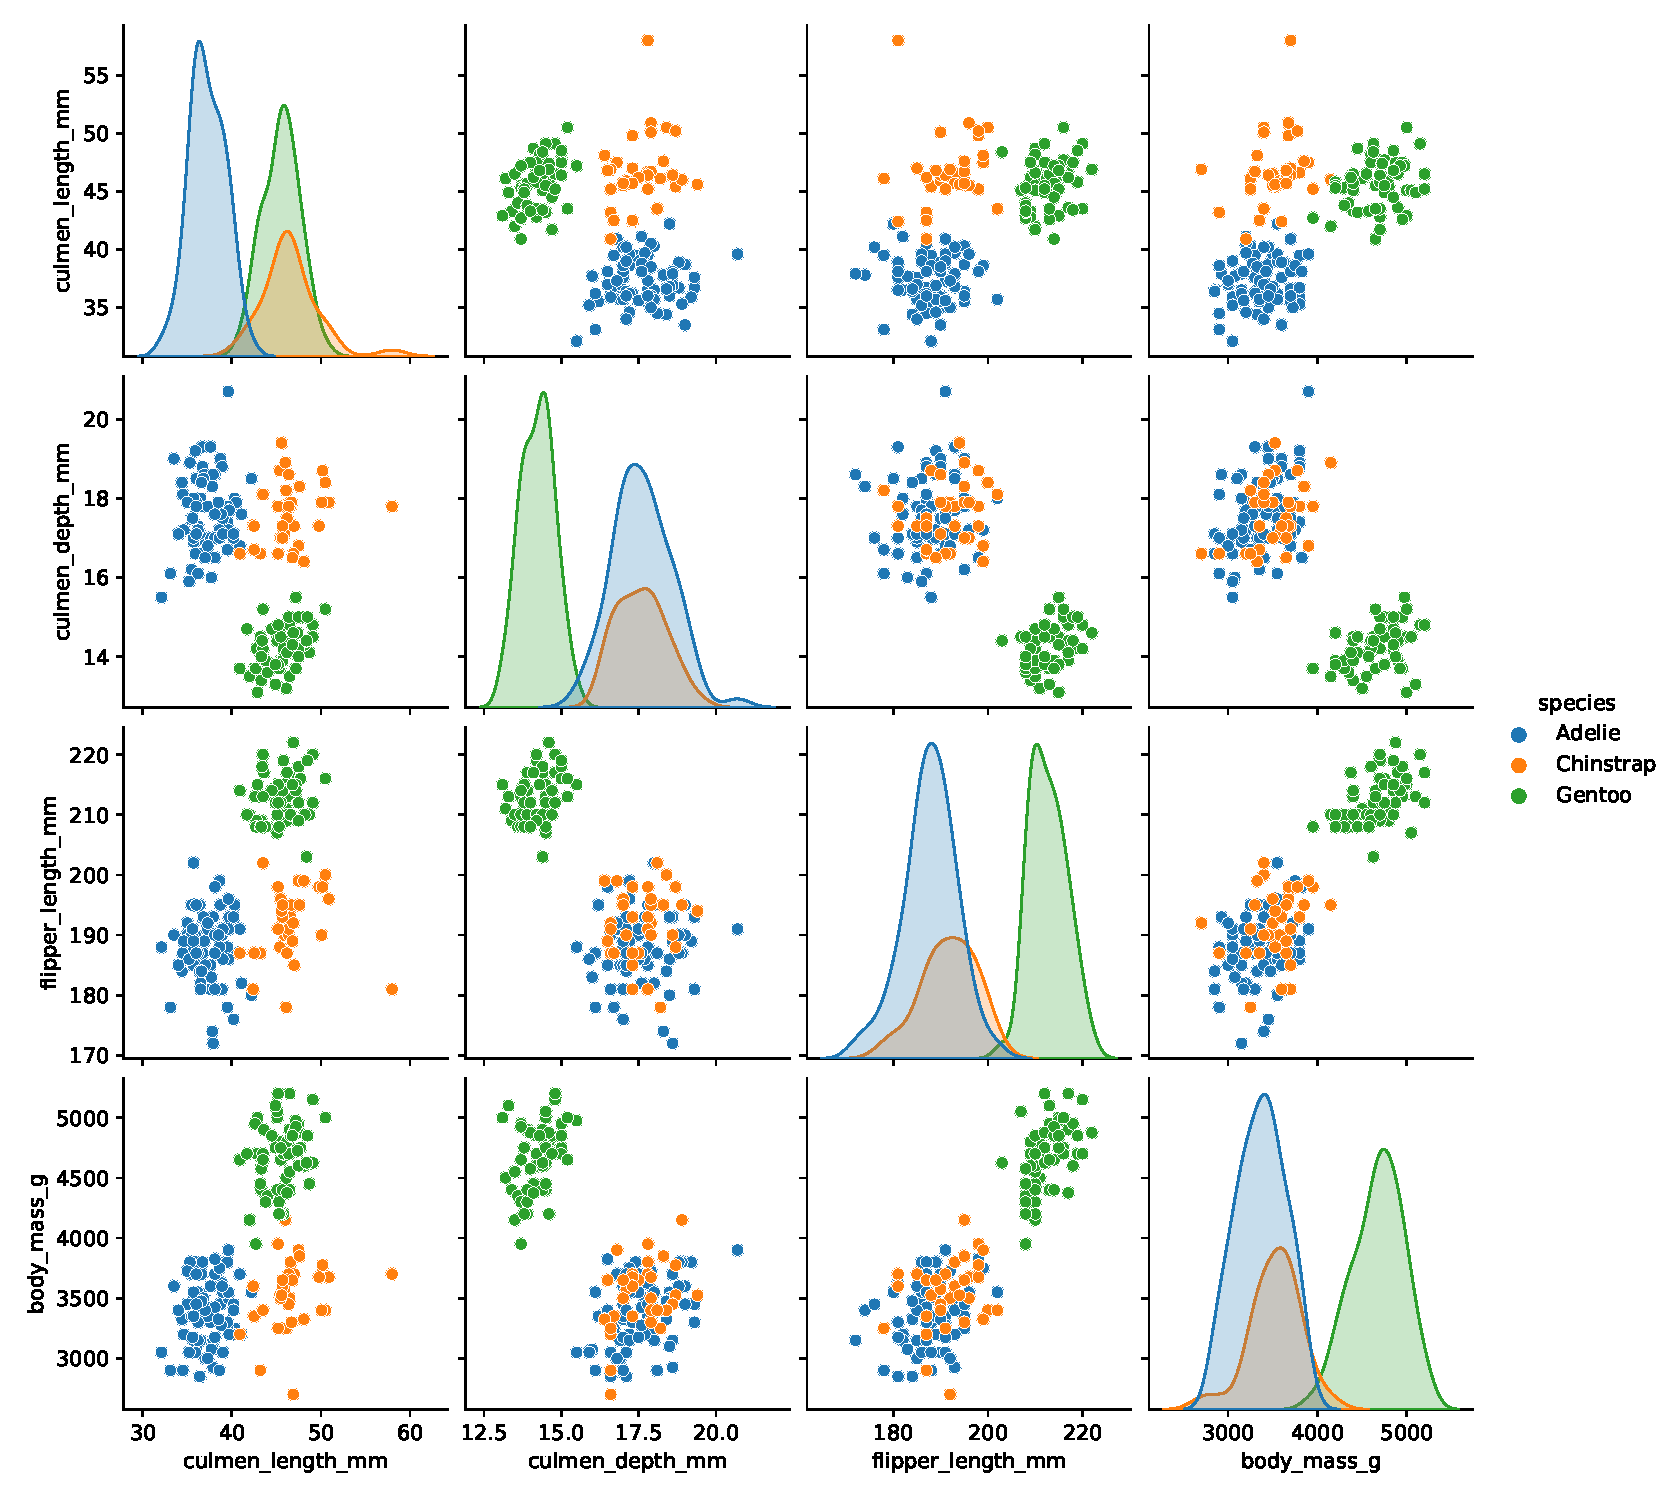
\includegraphics[width=1.0\textwidth, angle = 0]{img/female.pdf}
\subsubsection{Podrobnější rozložení numerických atributů v závisloti na pohlaví - Male}
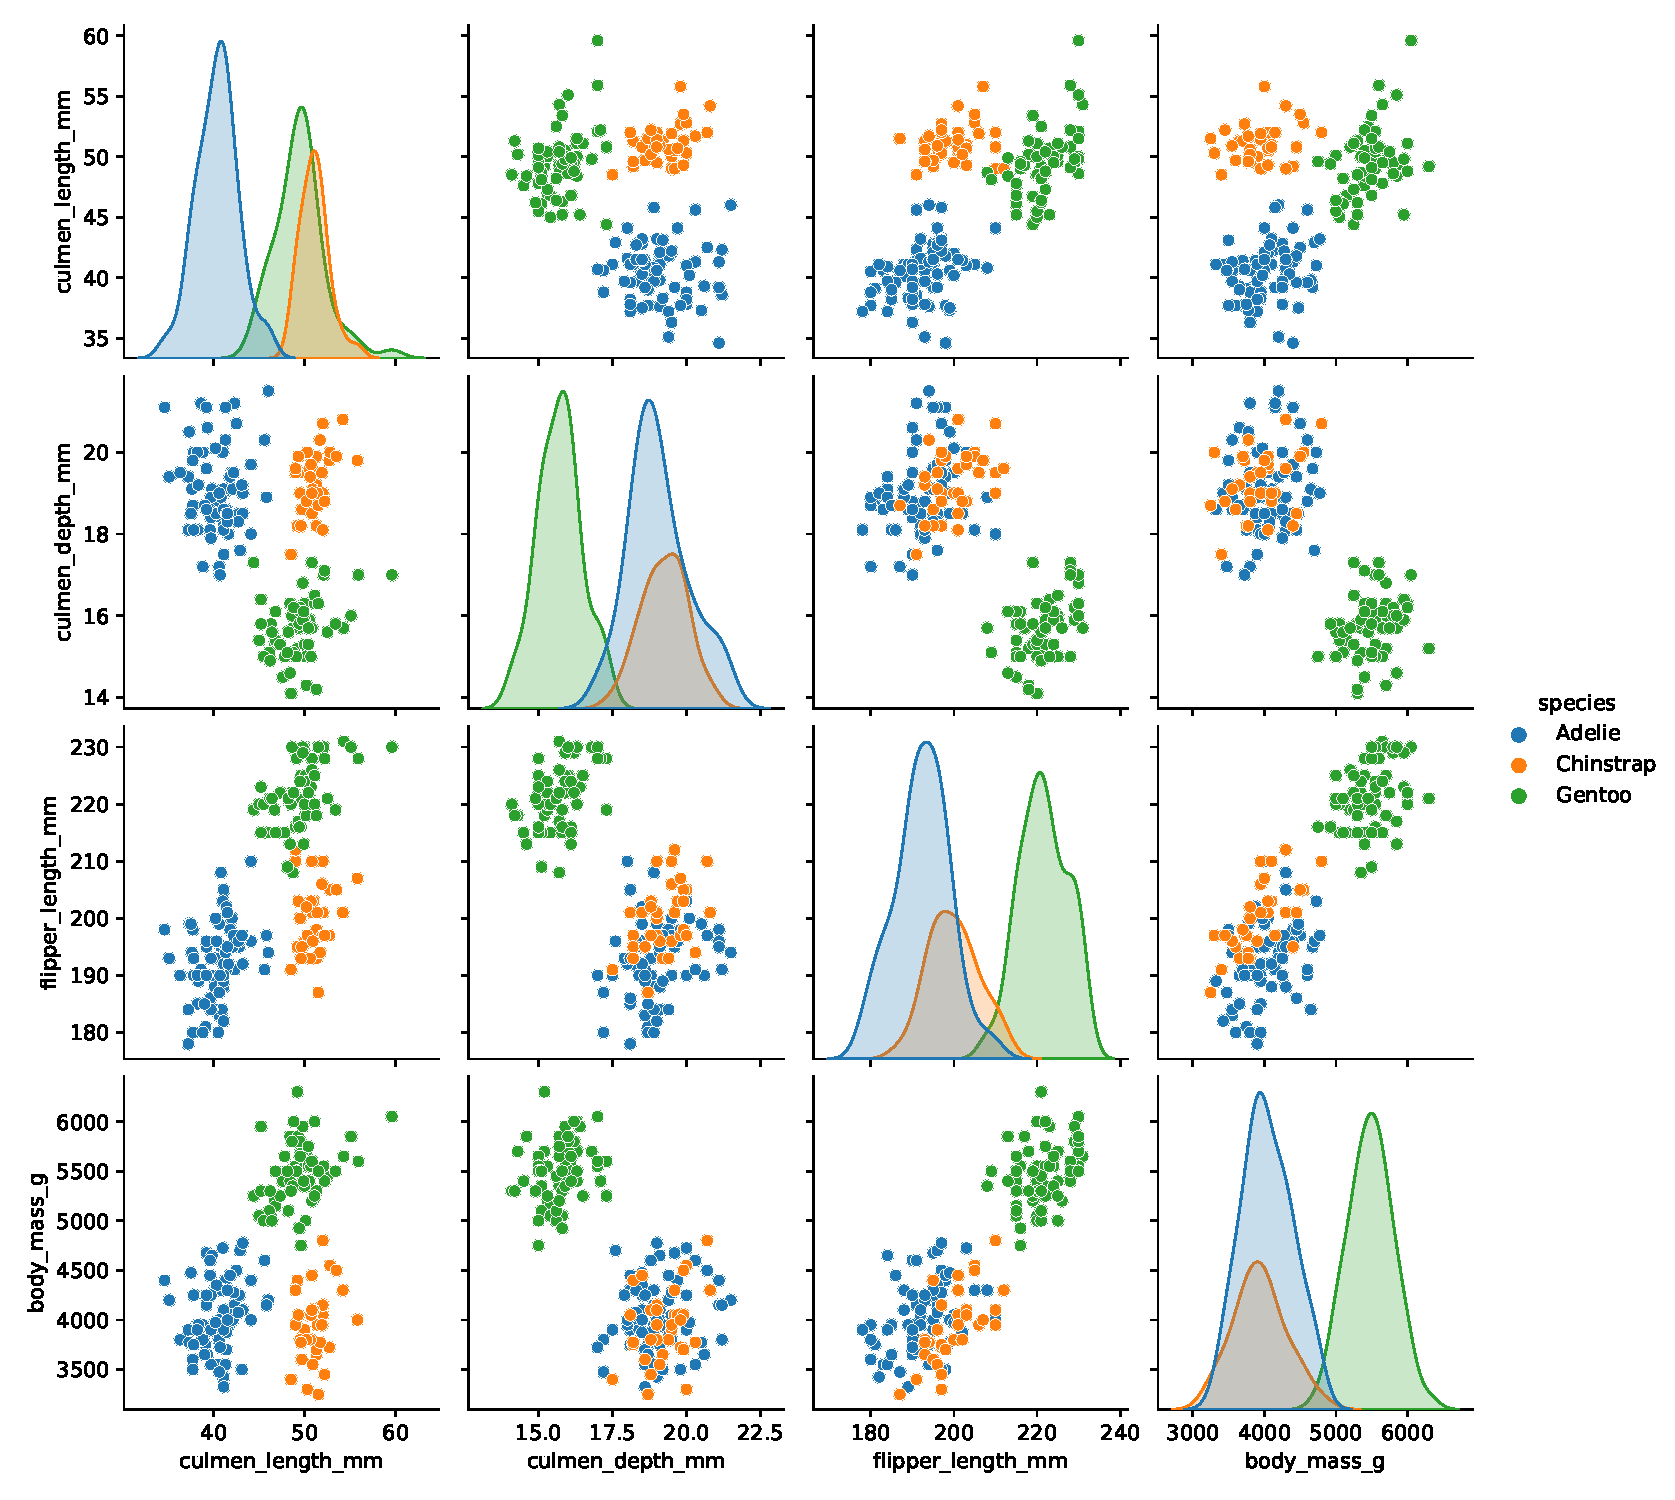
\includegraphics[width=1.0\textwidth, angle = 0]{img/male.pdf}

\section{Odlehlé hodnoty}
Několik odlehlých hodnot jde vyčíst z krabicového grafu v předešlé kapitoly.
\begin{itemize}
    \item 1 hodnota pro culmen length druhu Gentoo
    \item 1 hodnota pro culmen depth druhu Adelie
    \item 2 hodnoty pro flipper length druhu Adelie
    \item 2 hodnoty pro body mass druhu Chinstrap
\end{itemize}
Další odlehlé hodnoty lze identifikovat v maticových grafech a to především pro Female v řádku culmen length.

\section{Chybějící hodnoty}
\vspace{1em}
\begin{tabular}{|l|l|}
    \hline
    Atribut & Počet \\
    \hline
    \hline
    species           &  0 \\
    island            &  0 \\
    culmen length mm  &  2 \\
    culmen depth mm   &  2 \\
    flipper length mm &  2 \\
    body mass g       &  2 \\
    sex               & 10 \\
    \hline
\end{tabular}

\subsubsection{Jednotlivé řádky s chybjejícími hodnotami}
\vspace{1em}
\begin{tabular}{|l|l|}
    \hline
    \multicolumn{2}{|c|}{Řádek 3} \\
    \hline
    \hline
    Atribut & Počet \\
    \hline
    \hline
    species           &    Adelie \\
    island            & Torgersen \\
    culmen length mm  &       NaN \\
    culmen depth mm   &       NaN \\
    flipper length mm &       NaN \\
    body mass g       &       NaN \\
    sex               &       NaN \\
    \hline
\end{tabular}
\begin{tabular}{|l|l|}
    \hline
    \multicolumn{2}{|c|}{Řádek 8} \\
    \hline
    \hline
    Atribut & Počet \\
    \hline
    \hline
    species           &    Adelie \\
    island            & Torgersen \\
    culmen length mm  &      34.1 \\
    culmen depth mm   &      18.1 \\
    flipper length mm &     193.0 \\
    body mass g       &    3475.0 \\
    sex               &       NaN \\
    \hline
\end{tabular}
\begin{tabular}{|l|l|}
    \hline
    \multicolumn{2}{|c|}{Řádek 9} \\
    \hline
    \hline
    Atribut & Počet \\
    \hline
    \hline
    species           &    Adelie \\
    island            & Torgersen \\
    culmen length mm  &      42.0 \\
    culmen depth mm   &      20.2 \\
    flipper length mm &     190.0 \\
    body mass g       &    4250.0 \\
    sex               &       NaN \\
    \hline
\end{tabular}
\begin{tabular}{|l|l|}
    \hline
    \multicolumn{2}{|c|}{Řádek 10} \\
    \hline
    \hline
    Atribut & Počet \\
    \hline
    \hline
    species           &    Adelie \\
    island            & Torgersen \\
    culmen length mm  &      37.8 \\
    culmen depth mm   &      17.1 \\
    flipper length mm &     186.0 \\
    body mass g       &    3300.0 \\
    sex               &       NaN \\
    \hline
\end{tabular}
\begin{tabular}{|l|l|}
    \hline
    \multicolumn{2}{|c|}{Řádek 11} \\
    \hline
    \hline
    Atribut & Počet \\
    \hline
    \hline
    species           &    Adelie \\
    island            & Torgersen \\
    culmen length mm  &      37.8 \\
    culmen depth mm   &      17.3 \\
    flipper length mm &     180.0 \\
    body mass g       &    3700.0 \\
    sex               &       NaN \\
    \hline
\end{tabular}
\begin{tabular}{|l|l|}
    \hline
    \multicolumn{2}{|c|}{Řádek 47} \\
    \hline
    \hline
    Atribut & Počet \\
    \hline
    \hline
    species           & Adelie \\
    island            &  Dream \\
    culmen length mm  &   37.5 \\
    culmen depth mm   &   18.9 \\
    flipper length mm &  179.0 \\
    body mass g       & 2975.0 \\
    sex               &    NaN \\
    \hline
\end{tabular}
\begin{tabular}{|l|l|}
    \hline
    \multicolumn{2}{|c|}{Řádek 246} \\
    \hline
    \hline
    Atribut & Počet \\
    \hline
    \hline
    species           & Gentoo \\
    island            & Biscoe \\
    culmen length mm  &   44.5 \\
    culmen depth mm   &   14.3 \\
    flipper length mm &  216.0 \\
    body mass g       & 4100.0 \\
    sex               &    NaN \\
    \hline
\end{tabular}
\begin{tabular}{|l|l|}
    \hline
    \multicolumn{2}{|c|}{Řádek 286} \\
    \hline
    \hline
    Atribut & Počet \\
    \hline
    \hline
    species           & Gentoo \\
    island            & Biscoe \\
    culmen length mm  &   46.2 \\
    culmen depth mm   &   14.4 \\
    flipper length mm &  214.0 \\
    body mass g       & 4650.0 \\
    sex               &    NaN \\
    \hline
\end{tabular}
\begin{tabular}{|l|l|}
    \hline
    \multicolumn{2}{|c|}{Řádek 324} \\
    \hline
    \hline
    Atribut & Počet \\
    \hline
    \hline
    species           & Gentoo \\
    island            & Biscoe \\
    culmen length mm  &   47.3 \\
    culmen depth mm   &   13.8 \\
    flipper length mm &  216.0 \\
    body mass g       & 4725.0 \\
    sex               &    NaN \\
    \hline
\end{tabular}
\begin{tabular}{|l|l|}
    \hline
    \multicolumn{2}{|c|}{Řádek 339} \\
    \hline
    \hline
    Atribut & Počet \\
    \hline
    \hline
    species           & Gentoo \\
    island            & Biscoe \\
    culmen length mm  &    NaN \\
    culmen depth mm   &    NaN \\
    flipper length mm &    NaN \\
    body mass g       &    NaN \\
    sex               &    NaN \\
    \hline
\end{tabular}

\section{Korelační analýza}
Korelace je znázorně kombinací indexů a grafu typu heatmap. Tyto grafy jsou rozděleny podle druhu, ostrova a pohlaví.

\vspace{1em}
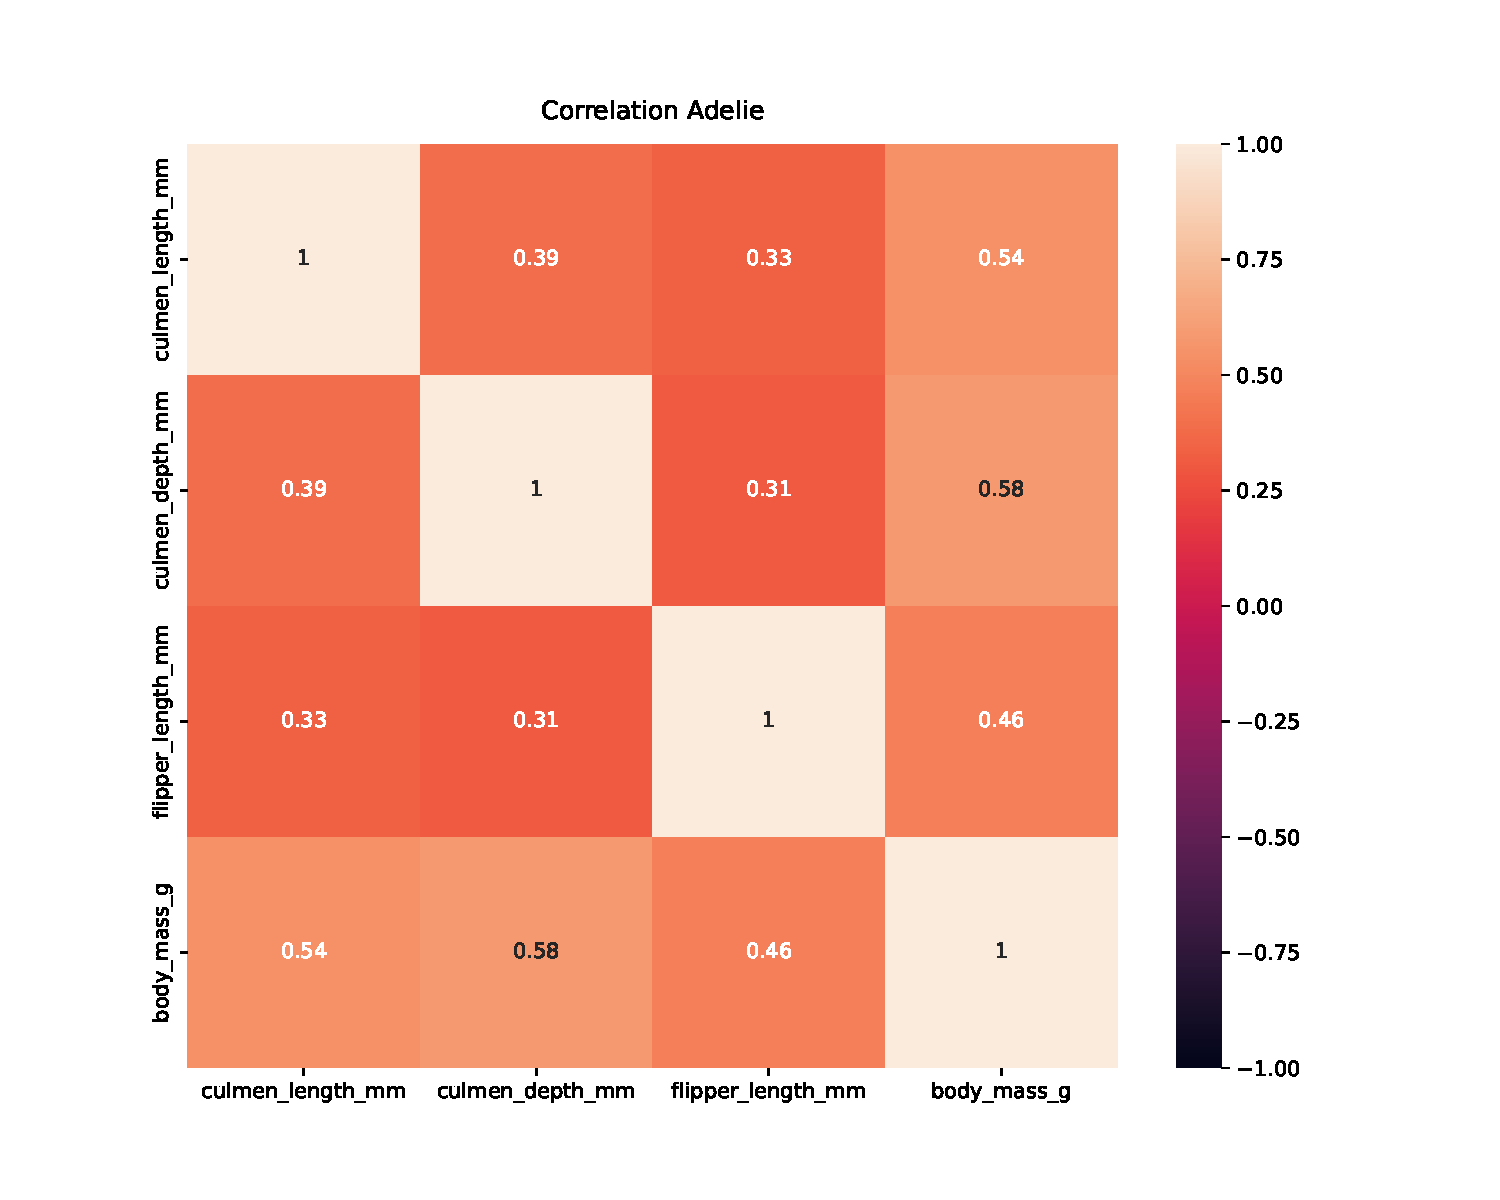
\includegraphics[width=0.65\textwidth, angle = 0]{img/adelie-corr.pdf}
\includegraphics[width=0.65\textwidth, angle = 0]{img/chinstrap-corr.pdf}
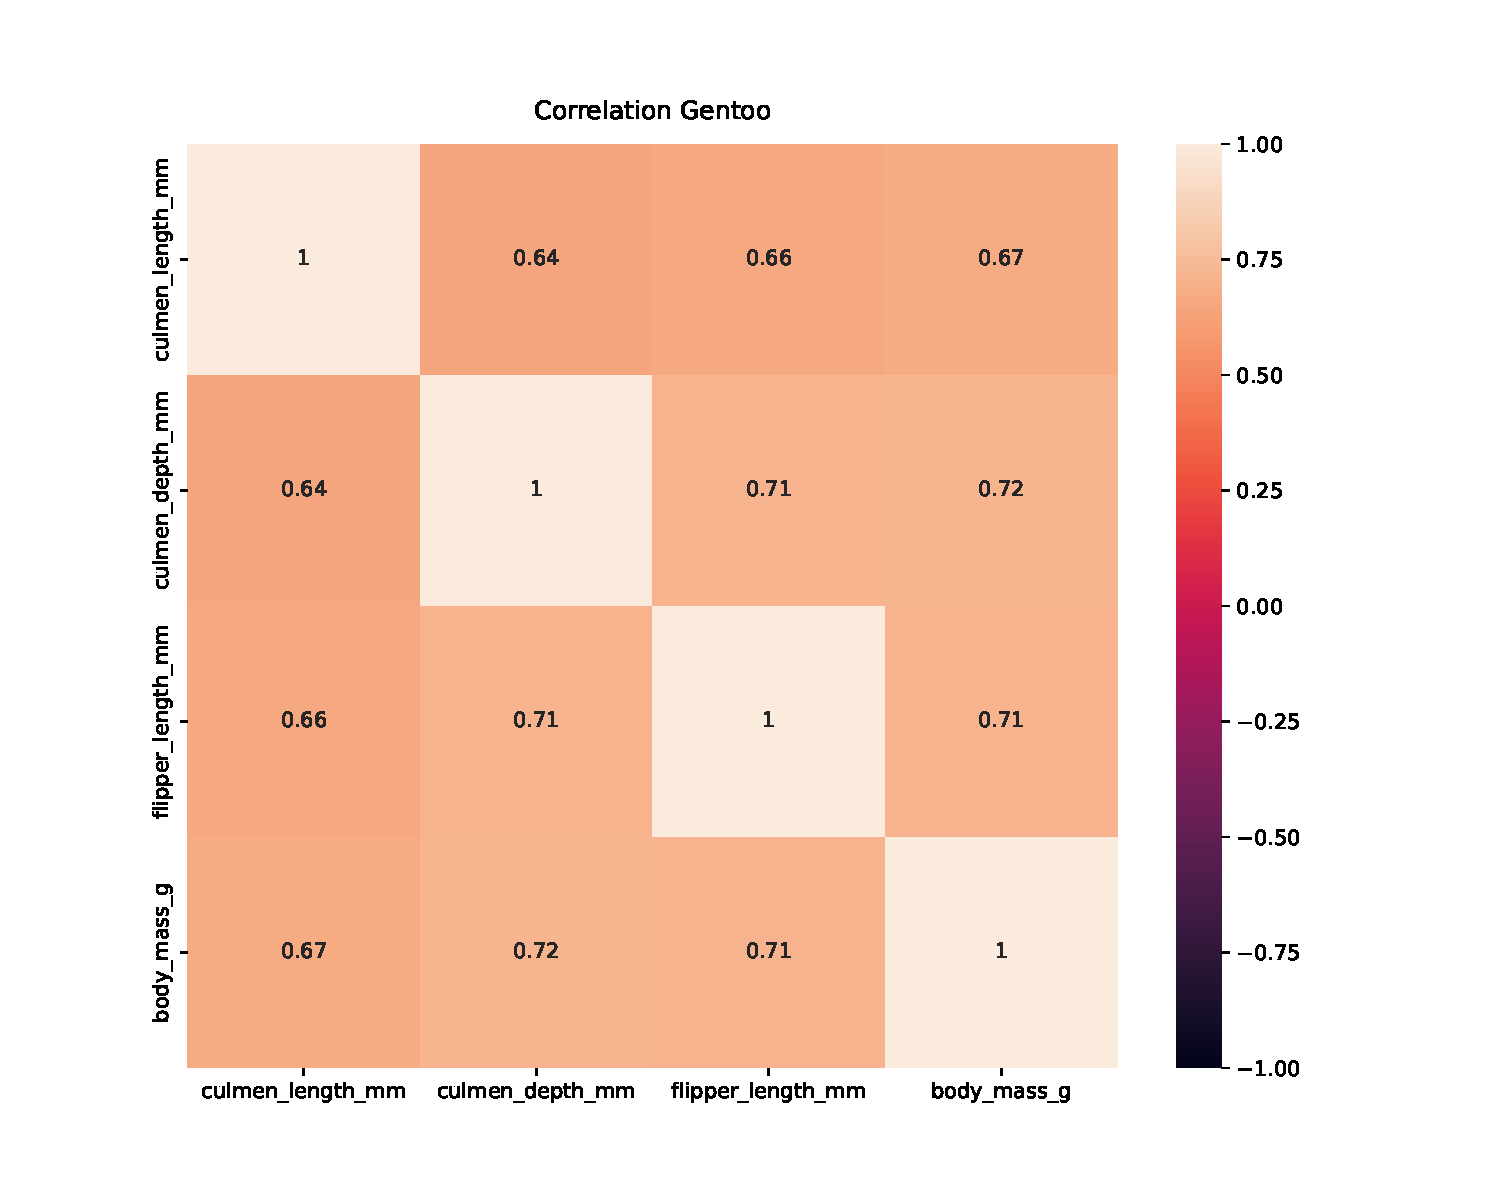
\includegraphics[width=0.65\textwidth, angle = 0]{img/gentoo-corr.pdf}
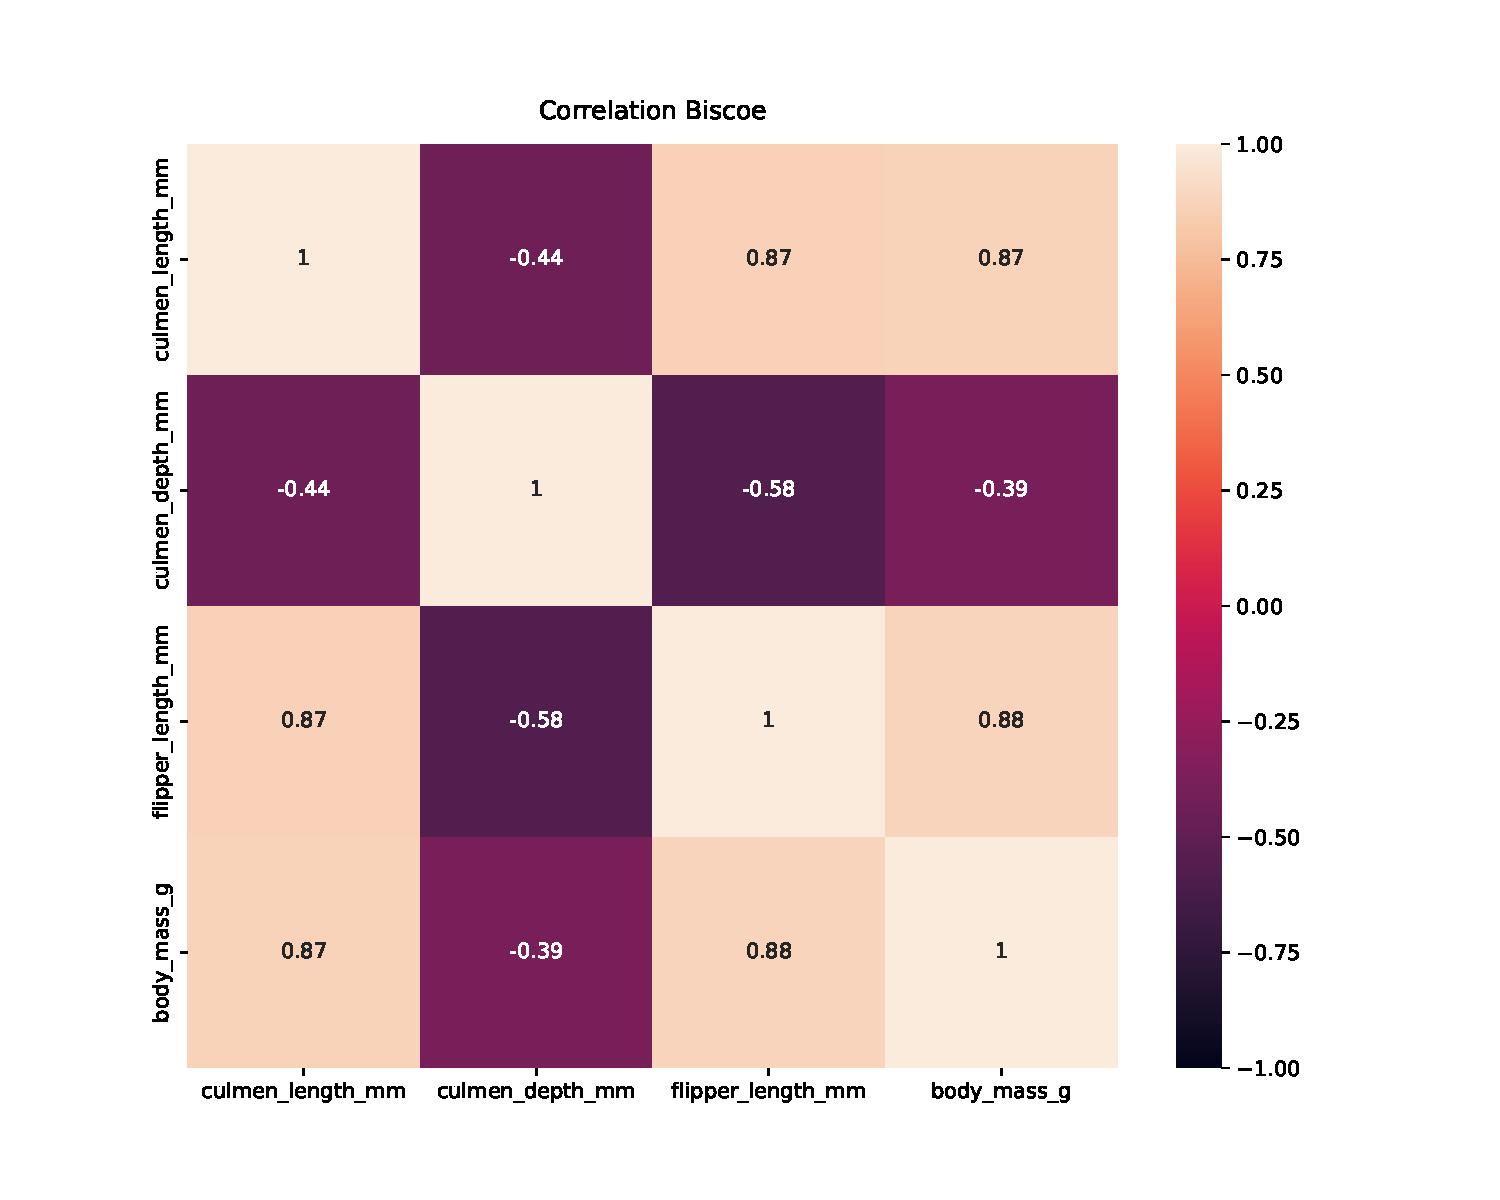
\includegraphics[width=0.65\textwidth, angle = 0]{img/biscoe-corr.pdf}
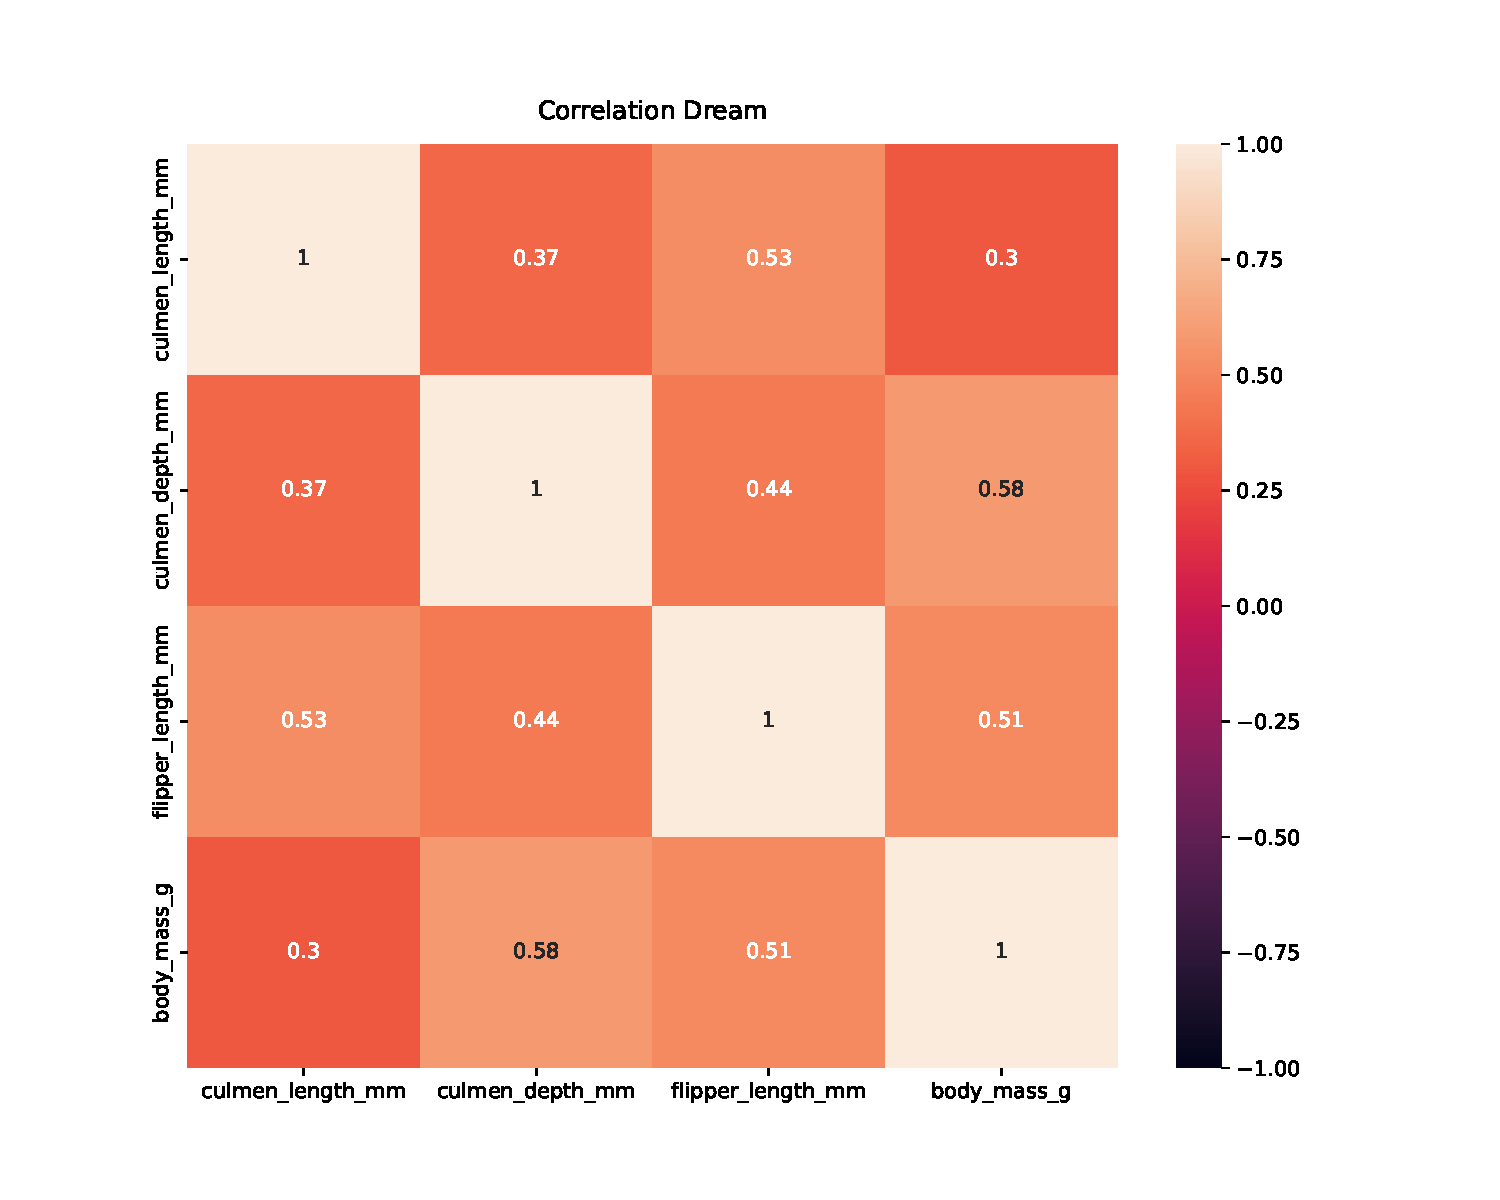
\includegraphics[width=0.65\textwidth, angle = 0]{img/dream-corr.pdf}
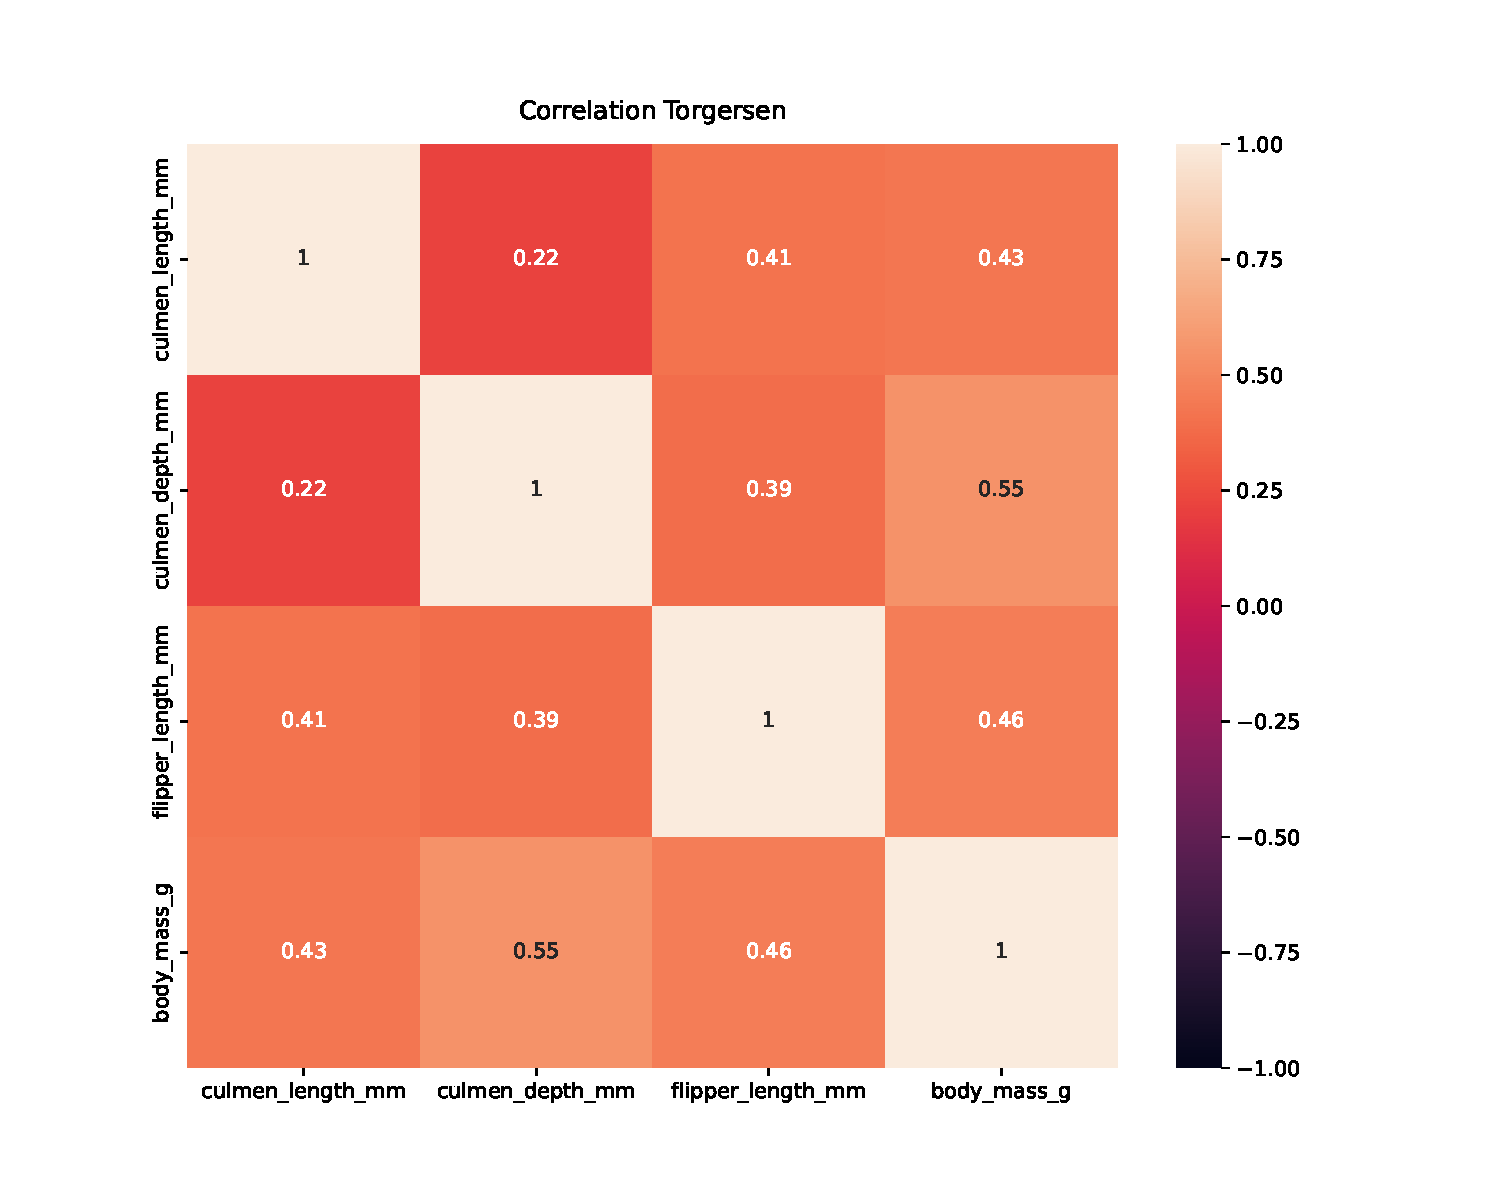
\includegraphics[width=0.65\textwidth, angle = 0]{img/torgersen-corr.pdf}
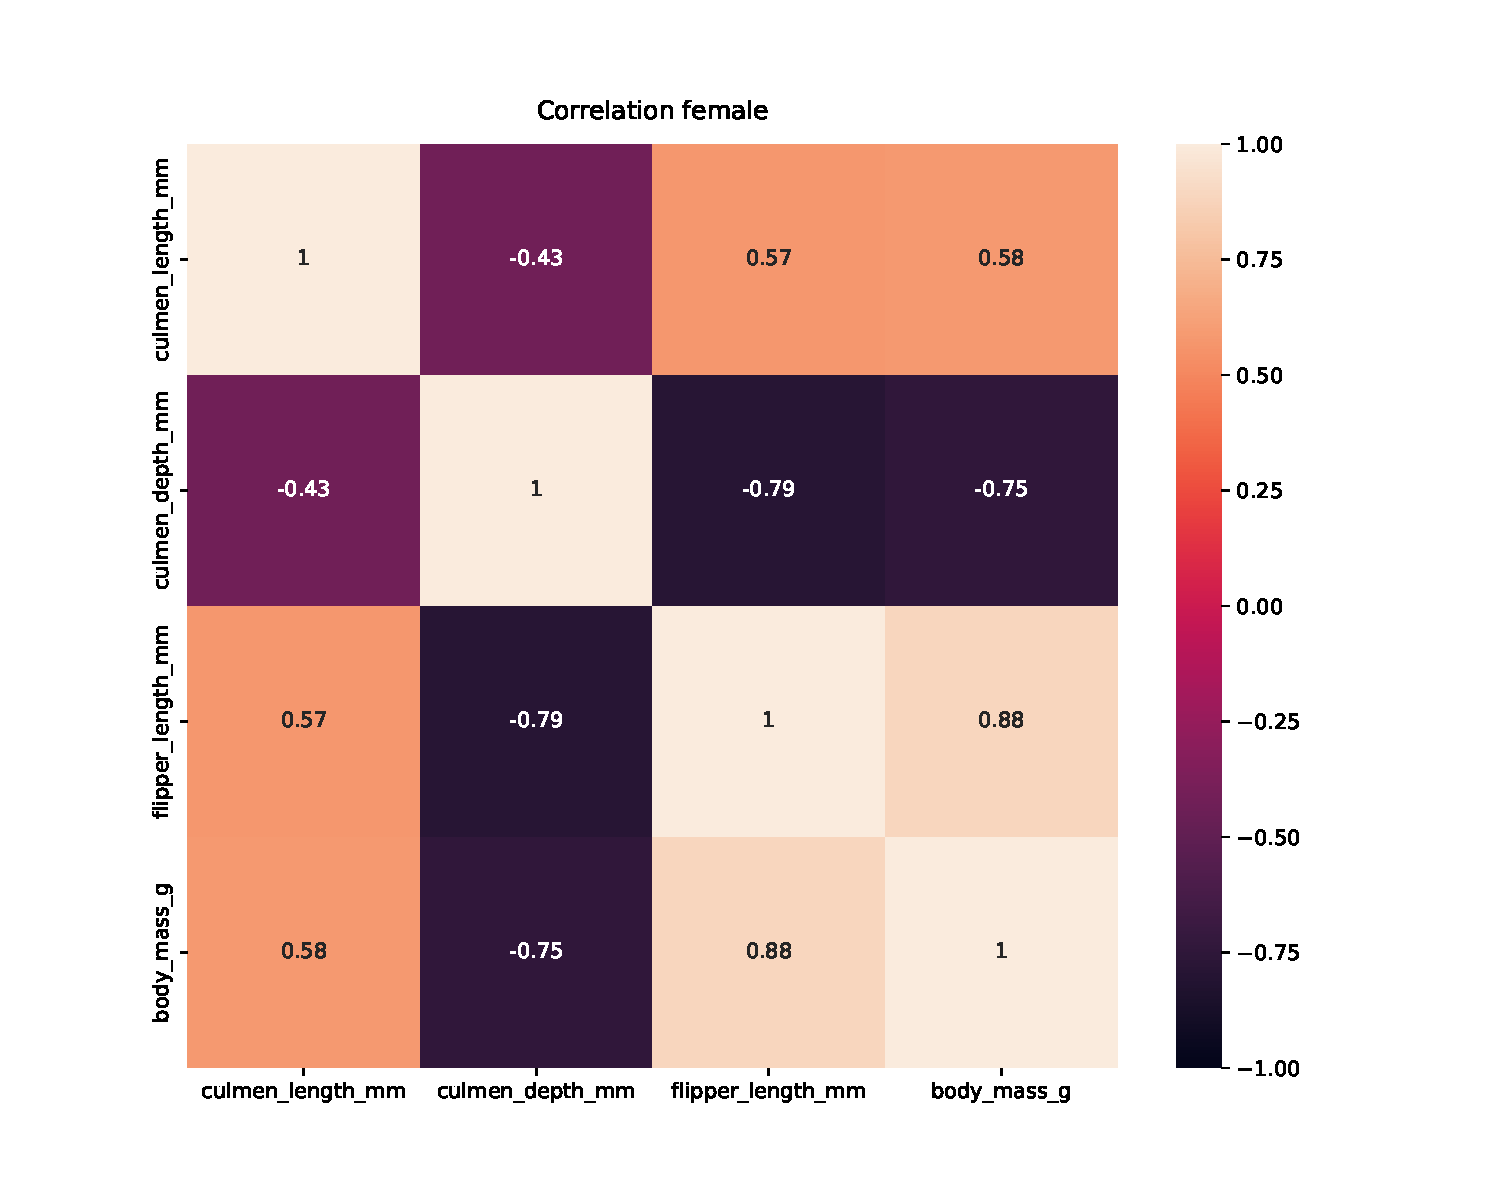
\includegraphics[width=0.65\textwidth, angle = 0]{img/female-corr.pdf}
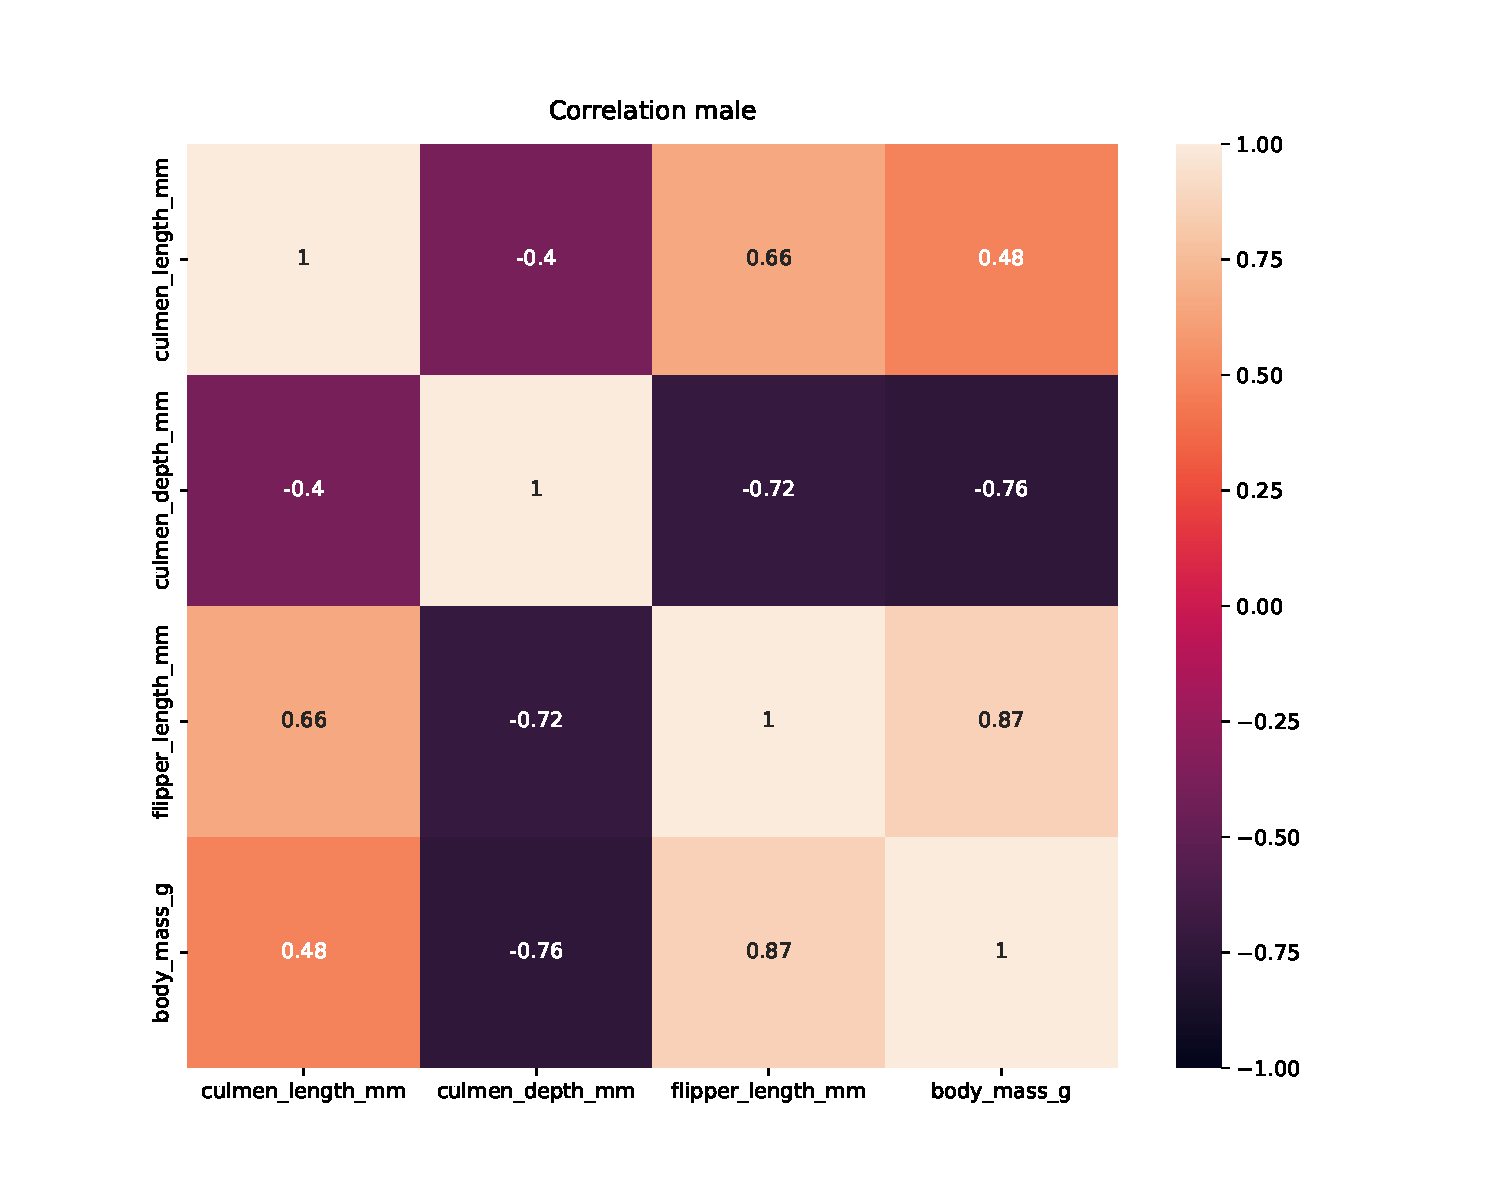
\includegraphics[width=0.65\textwidth, angle = 0]{img/male-corr.pdf}

% DOKUMENTACE K DRUHE CASTI DRUHEHO PROJEKTU
\chapter{Příprava datové sady}

\section{Zadání}
Datovou sadu obsahující informace o~tučňácích (\verb|penguins_lter.csv|) je třeba transformovat do podoby vhodné pro
dolovací úlohu – klasifikace druhů tučňáků na základě ostatních atributů. Výstupem jsou dva nové datové
soubory – \verb|A.csv| je vhodný pro metody vyžadující kategorické atributy a \verb|B.csv| je vhodný pro metody
vyžadující numerické atributy.

\section{Nástroje}
Jako nástroj pro úpravu datové sady byl zvolen programovací jazyk Python s využitím knihovny Pandas.
Tato knihovna obsahuje spoustu užitečných nástrojů pro zpracování souborů formátu csv a~pro následnou
práci s~daty. Pandas není součástí základní instalace Pythonu, je třeba ji doinstalovat
příkazem \verb|pip install pandas|. Skript implementující přípravu datové sady je uložen v
souboru \verb|modify_data.py|. Skript vyžaduje tři vstupní argumenty – cestu k původní datové sadě, cestu
k výstupní sadě s kategorickými atributy a cestu k výstupní sadě s numerickými atributy.\

Příklad spuštění:\

\verb|py ./src/modify_data.py ./dataset/penguins_lter.csv A.csv B.csv|\

Případně pomocí Makefile:\

\verb|make modify|\

\section{Postup}
Zpracování dat je rozděleno na několik dílčích kroků, některé jsou společně pro obě varianty výstupů.
\subsection{Odstranění irelevantních atributů}
Jedná se o~odstranění sloupců, které nejsou relevantní pro klasifikaci druhu tučňáka. V tomto případě se
jedná například o~různé identifikátory – například identifikátor studia, číslo sběru a~individuální ID.
Dále byly odstraněny informace o~snůškách vajec, region, ostrov (byl ponechán u~kategorické verze) a~komentář.
Byly ponechány informace o~fyzikálních vlastnostech tučňáků, jejich pohlaví a~druhu.

\subsection{Řešení chybějících hodnot}
V záznamech nebylo mnoho případů chybějících hodnot, proto byly ve většině případů odstraněny, především
ty záznamy, ve kterých chyběly informace o~fyzikálních vlastnostech tučňáků, nebo jejich pohlaví. Ve zbytku
dat bylo několik záznamů, kde chyběly informace o~složení krve. Tyto atributy byly doplněny mediánovou
hodnotou příslušného sloupce.

\subsection{Řešení odlehlých hodnot}
V~jednom případě byla ve sloupci Sex chyba – byla zde byla tečka namísto obvyklých \verb|MALE| nebo \verb|FEMALE|. Tento
záznam byl proto odstraněn. Krom tohoto případu nebyly v~datech žádné další významně odlehlé hodnoty.

\subsection{Kategorizace numerických hodnot}
Pro datovou sadu A byly sloupce obsahující numerické hodnoty převedeny na kategorické hodnoty – konkrétně na
určité intervaly hodnot. Jedná se o~rozdělení dat do „košů“ (binning), kdy interval mezi minimální a maximální
hodnotou sloupce je rozdělen na několik stejně velkých intervalů. V~tomto případě bylo použito dvacet košů.
Touto metodou byly upraveny všechny sloupce obsahující numerické hodnoty. Výsledná datová sada je v~souboru \verb|A.csv|.

\subsection{Převod kategorických hodnot na numerické}
V případě datové sady B bylo zapotřebí provést převod kategorických dat na numerická data a normalizovat
vhodné sloupce. Sloupec specifikující druh tučňáka obsahuje tři různé druhy, ty byly nahrazeny čísly 1 2 a 3.
Obdobně byly hodnoty \verb|MALE| a \verb|FEMALE| ve sloupci \verb|Sex| nahrazeny za hodnoty 0 a 1. Na závěr byla
provedena min-max normalizace u~dat popisující složení krve, konkrétně byly hodnoty převedeny na rozsah mezi 0 a 1.
Díky této úpravě jsou ve výsledné datové sadě všechny hodnoty nezáporné. Výsledná datová sada je v~souboru \verb|B.csv|.

\end{document}
